\ifx\PREAMBLE\UnDef
\documentclass{beamer}
\usepackage{tikz}
\usepackage[english]{babel}
% or whatever

\usepackage[latin1]{inputenc}
% or whatever
\usepackage{xifthen}
\usepackage{bsymb}
\usepackage{eventB}

\newcommand{\always}{\mathop{\square}}
\newcommand{\eventually}{\mathop{\diamondsuit}}
\newcommand{\until}{\mathop{\mathcal{U}}}
\newcommand{\predP}{P}
\newcommand{\predQ}{Q}

\begin{document}
\else
\fi

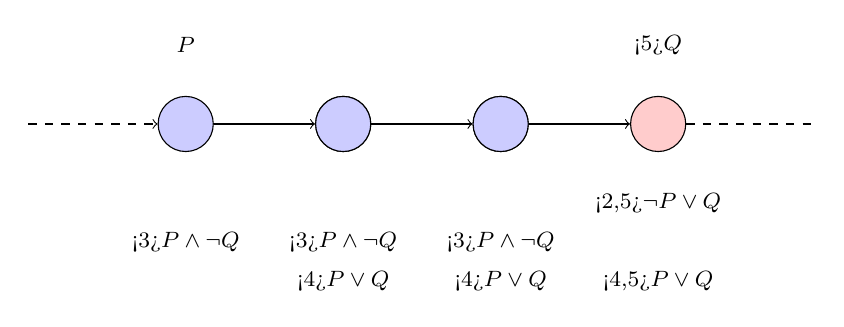
\begin{tikzpicture}[scale=1]
  \footnotesize
  \draw (0,0) node(s0)[circle, draw, inner sep =
  2pt, fill=blue!20!white, minimum width=0.7cm]{};
  \alt<1-2>{
    \draw (2,0) node(s1)[circle, draw, inner sep =
    2pt, fill=white!20!white, minimum width=0.7cm]{};
    \draw (4,0) node(s2)[circle, draw, inner sep =
    2pt, fill=white!20!white, minimum width=0.7cm]{};
  }
  {
    \draw (2,0) node(s1)[circle, draw, inner sep =
    2pt, fill=blue!20!white, minimum width=0.7cm]{};
    \draw (4,0) node(s2)[circle, draw, inner sep =
    2pt, fill=blue!20!white, minimum width=0.7cm]{};
  }
  \draw (6,0) node(s3)[circle, draw, inner sep =
  2pt, fill=red!20!white, minimum width=0.7cm]{};
  \draw[->,dashed] (-2,0) -- (s0);
  \draw[->] (s0) -- (s1);
  \draw[->] (s1) -- (s2);
  \draw[->] (s2) -- (s3);
  \draw[dashed] (s3) -- (8, 0);
  \draw (0,1) node{$\structure{\predP}$};
  \uncover<2->{\draw (6,-1) node{\alert<2,5>{$\neg \predP \lor \predQ$}};}
  \uncover<3->{
    \draw (4,-1.5) node{\alert<3>{$\predP \land \neg \predQ$}};
    \draw (2,-1.5) node{\alert<3>{$\predP \land \neg \predQ$}};
    \draw (0,-1.5) node{\alert<3>{$\predP \land \neg \predQ$}};
  }
  \uncover<4->{
    \draw (2, -2) node{\alert<4>{$\predP \lor \predQ$}};
    \draw (4, -2) node{\alert<4>{$\predP \lor \predQ$}};
    \draw (6, -2) node{\alert<4,5>{$\predP \lor \predQ$}};
  }
  % \uncover<4->{
  %   \draw (4,1) node{\structure{$\predP$}};
  %   \draw (2,1) node{\structure{$\predP$}};
  % }
  \uncover<5->{
    \draw (6, 1) node{\alert<5>{$\predQ$}};
  }
\end{tikzpicture}

\ifx\PREAMBLE\UnDef
\end{document}
\else
\fi
